\subsection{Main Game Loop}
	 The Main Game Loop is the contains the main function in which all game logic is performed. The game logic is performed using the classes described above. The following class diagram, figure \ref{fig:classMain}, shows the dependencies for the Main Game Loop. 

	\begin{figure}[H]
		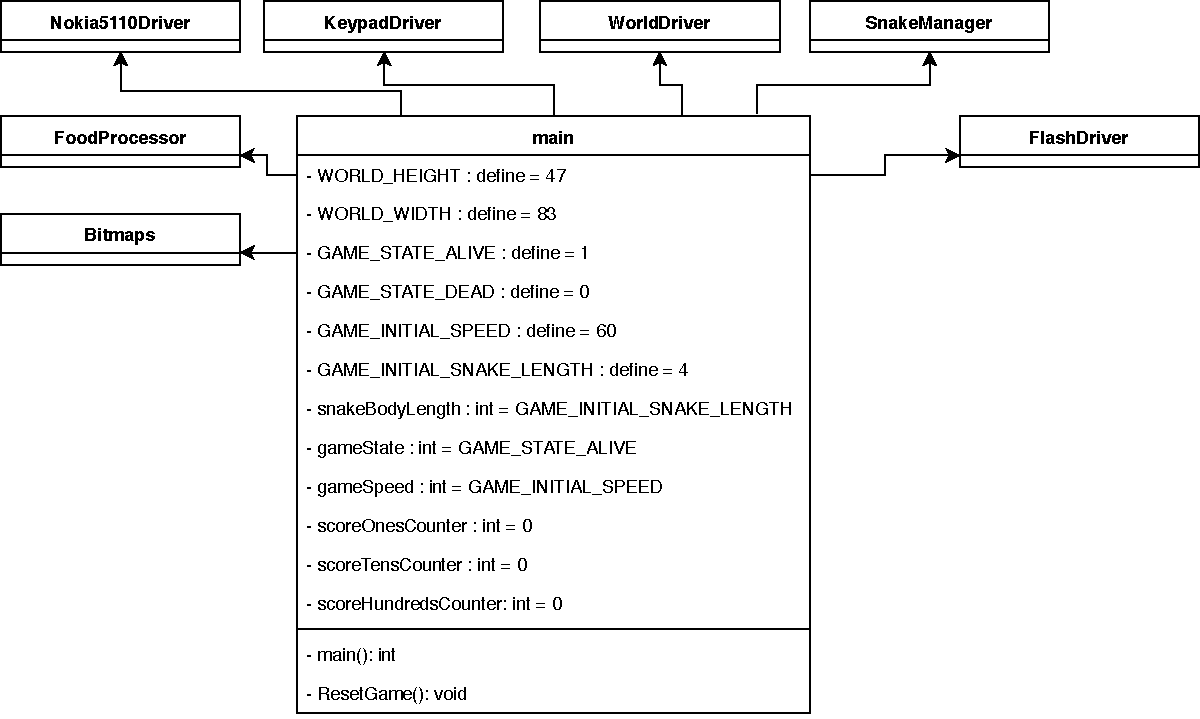
\includegraphics[width=14cm]{MainClassDiagram}
		\centering
		\caption{Class diagram for MainGameLoop}
		\label{fig:classMain}
	\end{figure}
	
	\begin{table}[H]
		\centering
		\begin{tabular}{|l|l|}
			\hline
			\multicolumn{1}{|c|}{\textbf{Method}} & \multicolumn{1}{c|}{\textbf{Description}} \\ \hline
			main & \begin{tabular}[c]{@{}l@{}}This method contains all game logic.\\ This includes initializing hardware\\ components, food collision detection,\\ game rendering and displaying data.\end{tabular} \\ \hline
			ResetGame & \begin{tabular}[c]{@{}l@{}}This method contains logic to reset\\ the game. This includes resetting \\speed, length and score values.\end{tabular} \\ \hline
		\end{tabular}
		\caption{Description of the methods of MainGameLoop}
		\label{fig:methodsMGL}
	\end{table}

	\begin{table}[H]
		\centering
		\begin{tabular}{|l|l|}
			\hline
			\multicolumn{1}{|c|}{\textbf{Attribute}} & \multicolumn{1}{c|}{\textbf{Description}} \\ \hline
			\begin{tabular}[c]{@{}l@{}}WORLD\_HEIGHT/\\ WORLD\_WIDTH\end{tabular} & \begin{tabular}[c]{@{}l@{}}These attributes describe the pixel dimensions for the \\Nokia 5110 Display.\end{tabular} \\ \hline
			\begin{tabular}[c]{@{}l@{}}GAME\_STATE\_ALIVE/\\ GAME\_STATE\_DEAD\end{tabular} & These attributes describe the gamestate. \\ \hline
			\begin{tabular}[c]{@{}l@{}}GAME\_INITAL\_SPEED/\\ GAME\_INITIAL\_\\ SNAKE\_LENGTH\end{tabular} & \begin{tabular}[c]{@{}l@{}}These attributes describe inital values for the frame\\ rate of the display and for the length \\of the snake. When the game is reset the speed and \\length are reset to these values.\end{tabular} \\ \hline
			snakeBodyLength & \begin{tabular}[c]{@{}l@{}}Indicates the current length of the snake. This value\\ is incremented twice each time the snake collides with\\ food.\end{tabular} \\ \hline
			gameState & \begin{tabular}[c]{@{}l@{}}Indicates the current game state. This is used to \\determine if the game should be reset and if the high\\ score should be displayed.\end{tabular} \\ \hline
			gameSpeed & \begin{tabular}[c]{@{}l@{}}Indicates the frame rate of the display. This value\\ translates to the speed of the snake movement.\end{tabular} \\ \hline
			\begin{tabular}[c]{@{}l@{}}scoreOnesCounter/\\ scoreTensCounter/\\ scoreHundredsCounter\end{tabular} & \begin{tabular}[c]{@{}l@{}}Indicates the score which combined make up a three\\ digit score. The hundreds counter is not displayed and\\ is used to roll over the score if it exceeds 99.\end{tabular} \\ \hline
		\end{tabular}
		\caption{Description of the attributes of MainGameLoop}
		\label{my-label}
	\end{table}
	
	\textbf{Reset Logic} \newline
		The ResetGame method contains all reset logic to restore the game to the initial
		state. This includes resetting in-game values such as the state, score, length and speed. The display's cursor is reset and cleared, to ensure that the next rendering will start at the upper left hand corner, in case the game stops in the middle of a rendering. The display is cleared Additionally, this is where a new snake is created and a new food position is generated. This position will be used when the game restarts.
	
	\textbf{Food Collision Detection} \newline
	
	\textbf{World Rendering} \newline
		The main class of the game keeps track of the world through a char array of 504 bytes - a direct mapping to the DDRAM of the display. 
		This array contains the visual information to show the snake and food objects.
		In each gameloop, the array is updated with new positions for the snake and food, using the \textit{DrawDot()} and \textit{DrawFood()} methods of the worldDriver.
		At the end of the gameloop, the array is sent to the display using the \textit{RenderWorld()} method of the worldDriver.
		This has been depicted with pseudo-code in the sequence diagram on figure \ref{SnakeRenderLoop}.
		
		\begin{figure}[H]
			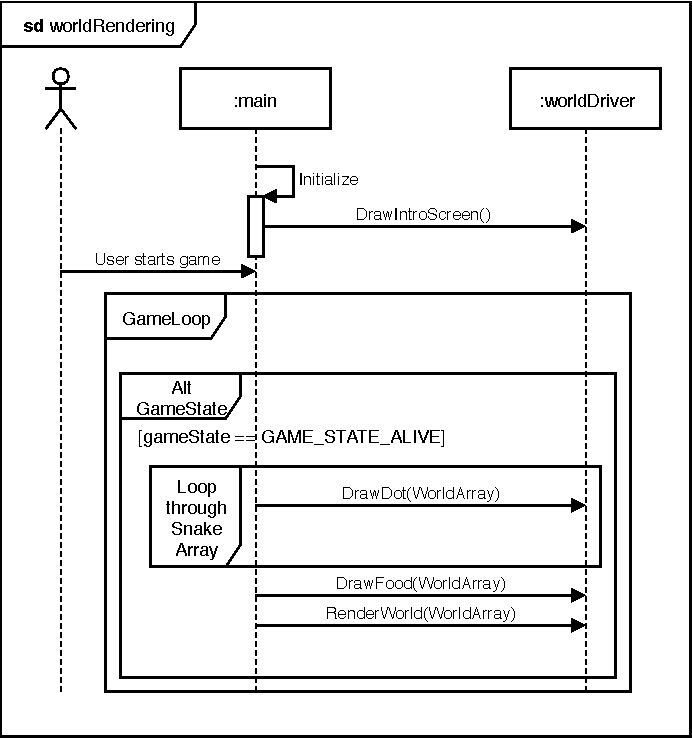
\includegraphics{SnakeRenderLoop}
			\centering
			\caption{Sequence of world rendering using pseudo-code.}
			\label{SnakeRenderLoop}
		\end{figure}
	
	\textbf{High Score Presentation} \newline
		When the snake collides with itself, the game is finished and the screen displays the high score header, defined in Bitmaps, and the current top 3 high scores. The following diagram shows the sequence for visualizing and updating the display.
		
			\begin{figure}[H]
				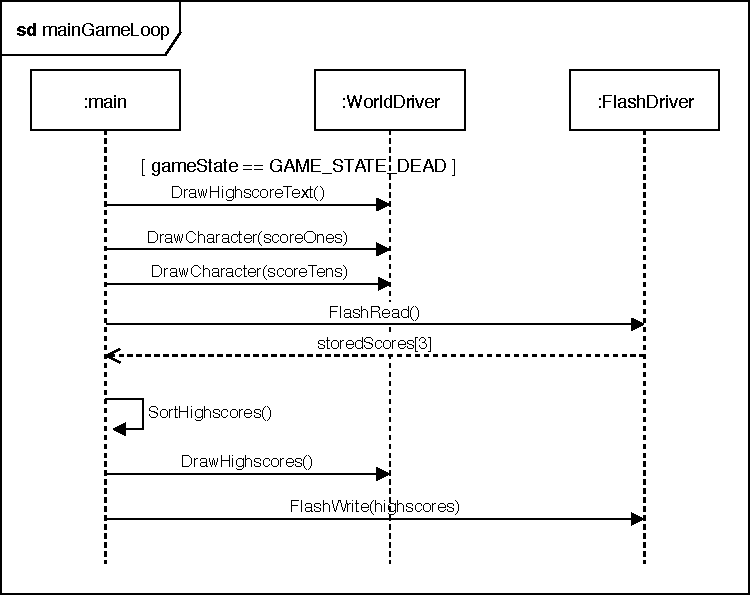
\includegraphics[width=14cm]{sequenceHighScore}
				\centering
				\caption{Class diagram for MainGameLoop}
				\label{fig:classMain}
			\end{figure}
		




